\documentclass{beamer}
\usepackage{beamerthemeshadow}
\usepackage{tabulary}
\usepackage{xcolor}
\usepackage{color}

\usepackage{mathtools}
\usepackage{amsmath}
\usepackage{graphicx}
\usepackage{lmodern}% http://ctan.org/pkg/lm

%\usepackage[mediumspace,mediumqspace,squaren]{SIunits}
\graphicspath{{../figures/}}

\usetheme{Copenhagen}
\usecolortheme{crane}
%\useinnertheme{circles}
\usefonttheme{structurebold}
\usefonttheme[onlymath]{serif}

%\usepackage[english]{babel}
%\usepackage[latin1]{inputenc}
%\usepackage{times}
%%\usepackage[T1]{fontenc}


\setbeamerfont{page number in head/foot}{size=\small}
\setbeamerfont{caption}{size=\tiny}
%\usepackage[textfont={big,it}]{caption}
\setbeamertemplate{footline}[frame number]

\beamersetuncovermixins{\opaqueness<1>{25}}{\opaqueness<2->{15}}
\usepackage{caption}
\captionsetup[figure]{labelformat=empty}% redef the caption setup
\begin{document}
\title{Digital Electronics Workshop} 
\author{Nik Dennler, Johannes Lade}
\date{\today} 

\begin{frame}
\titlepage
\end{frame} 

\begin{frame}\frametitle{Table of Contents}\tableofcontents
\end{frame} 


\section{Introduction}
\begin{frame}\frametitle{How does this work??}
  \begin{columns}
  \begin{column}{6cm}
  \begin{figure}
  
\includegraphics[width=1\textwidth]{witcher}
  \caption{3D Graphics}
  \end{figure}
  %\vspace{3cm} 
  \end{column}
  \begin{column}{6cm}
  \begin{figure}
  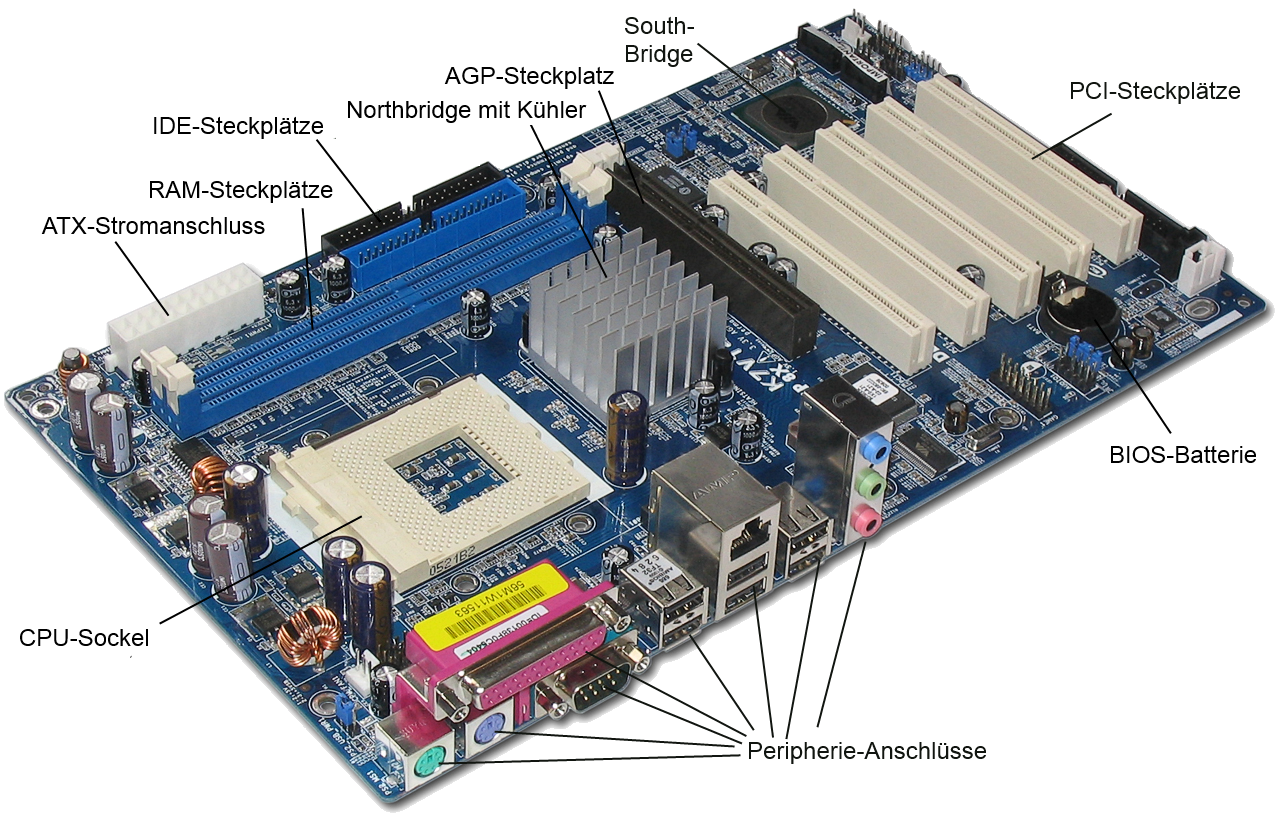
\includegraphics[width=1\textwidth]{motherboard}
  \caption{Motherboard}
  \end{figure}
  \end{column}
  \end{columns}
\end{frame}


\begin{frame}\frametitle{What do we need?}
  \centering
  Numbers!
  \begin{figure}
  
\includegraphics[width=0.7\textwidth]{numbers}

  \end{figure}

\end{frame}

\begin{frame}\frametitle{Now what do we do with it?}
  \begin{columns}
  \begin{column}{6cm}
  \begin{figure}
  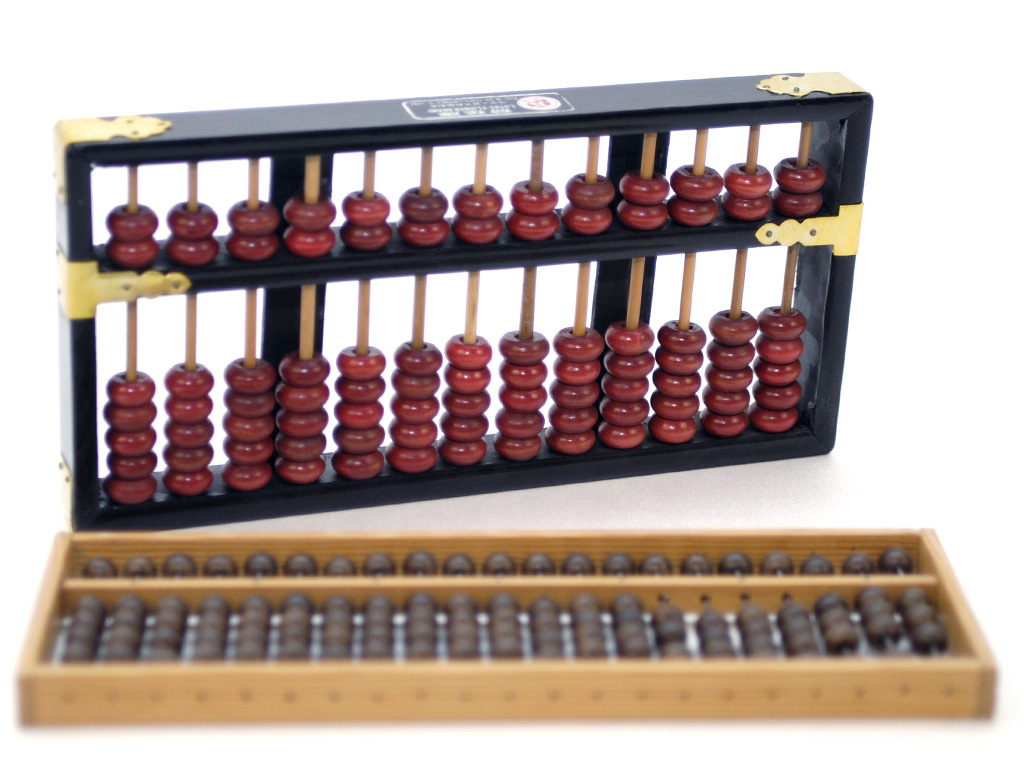
\includegraphics[width=1\textwidth]{abakus}
  \caption{Calculations}
  \end{figure}
  %\vspace{3cm} 
  \end{column}
  \begin{column}{6cm}
  \begin{figure}
  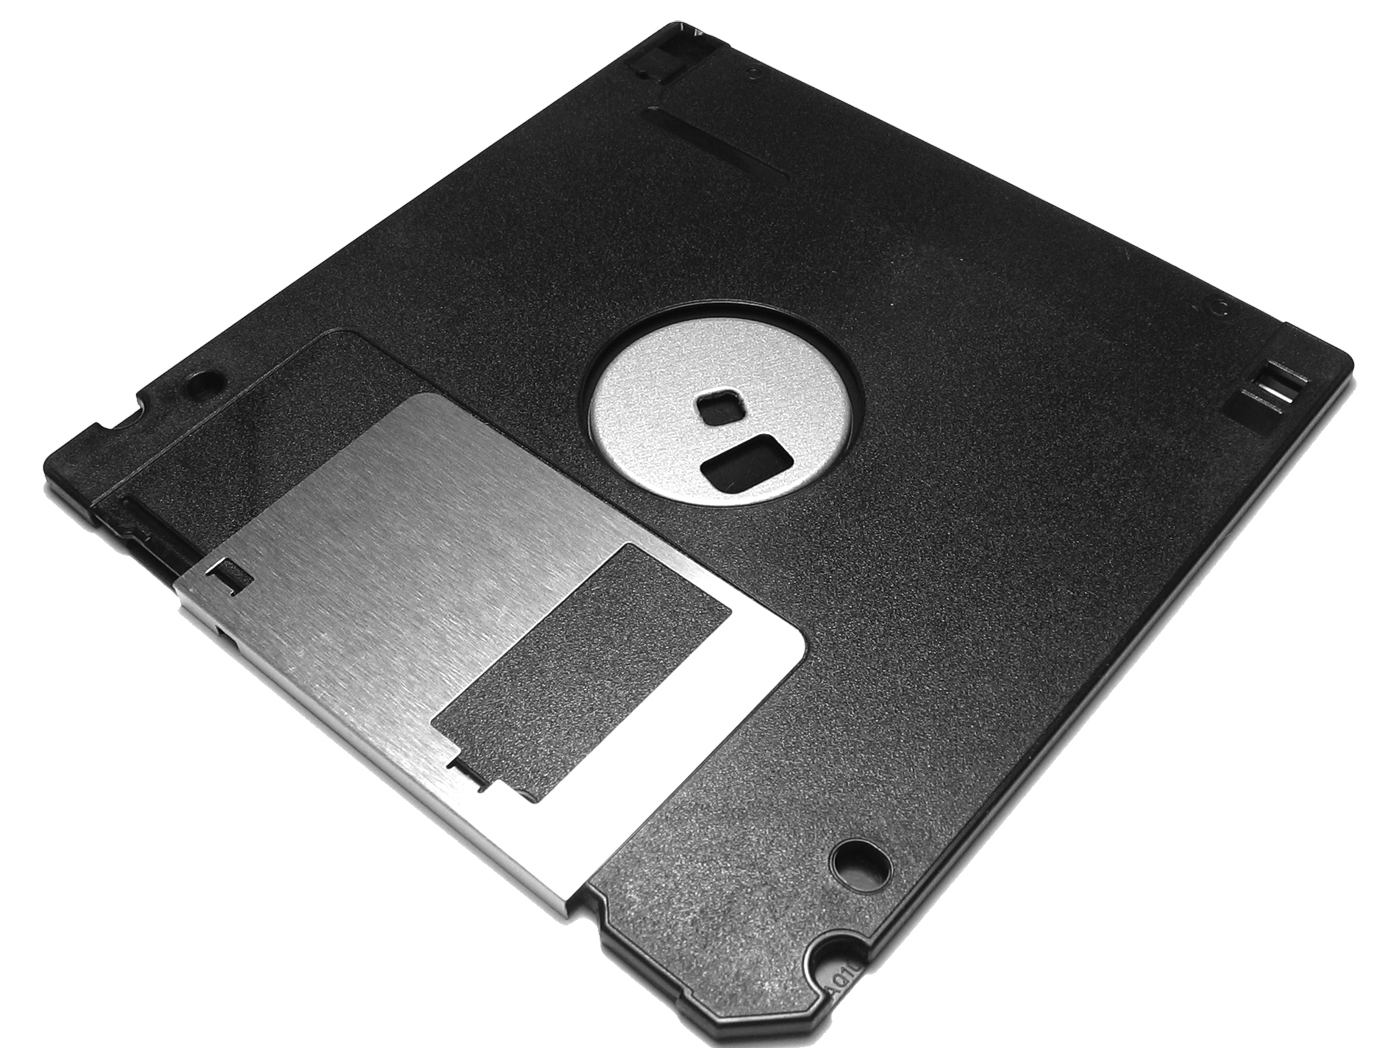
\includegraphics[width=1\textwidth]{memory}
  \caption{Memory}
  \end{figure}
  \end{column}
  \end{columns}
\end{frame}


\section{Digital Circuits}
\begin{frame}\frametitle{Analog Circuit}
  \begin{columns}
  \begin{column}{6cm}
  \begin{itemize}
   \item Continuous Voltage Levels
   \item Kirchhoff Ciruit Law's
   \item Example: Guitar Amplifier

  \end{itemize}


  \end{column}
  \begin{column}{6cm}
  \begin{figure}
  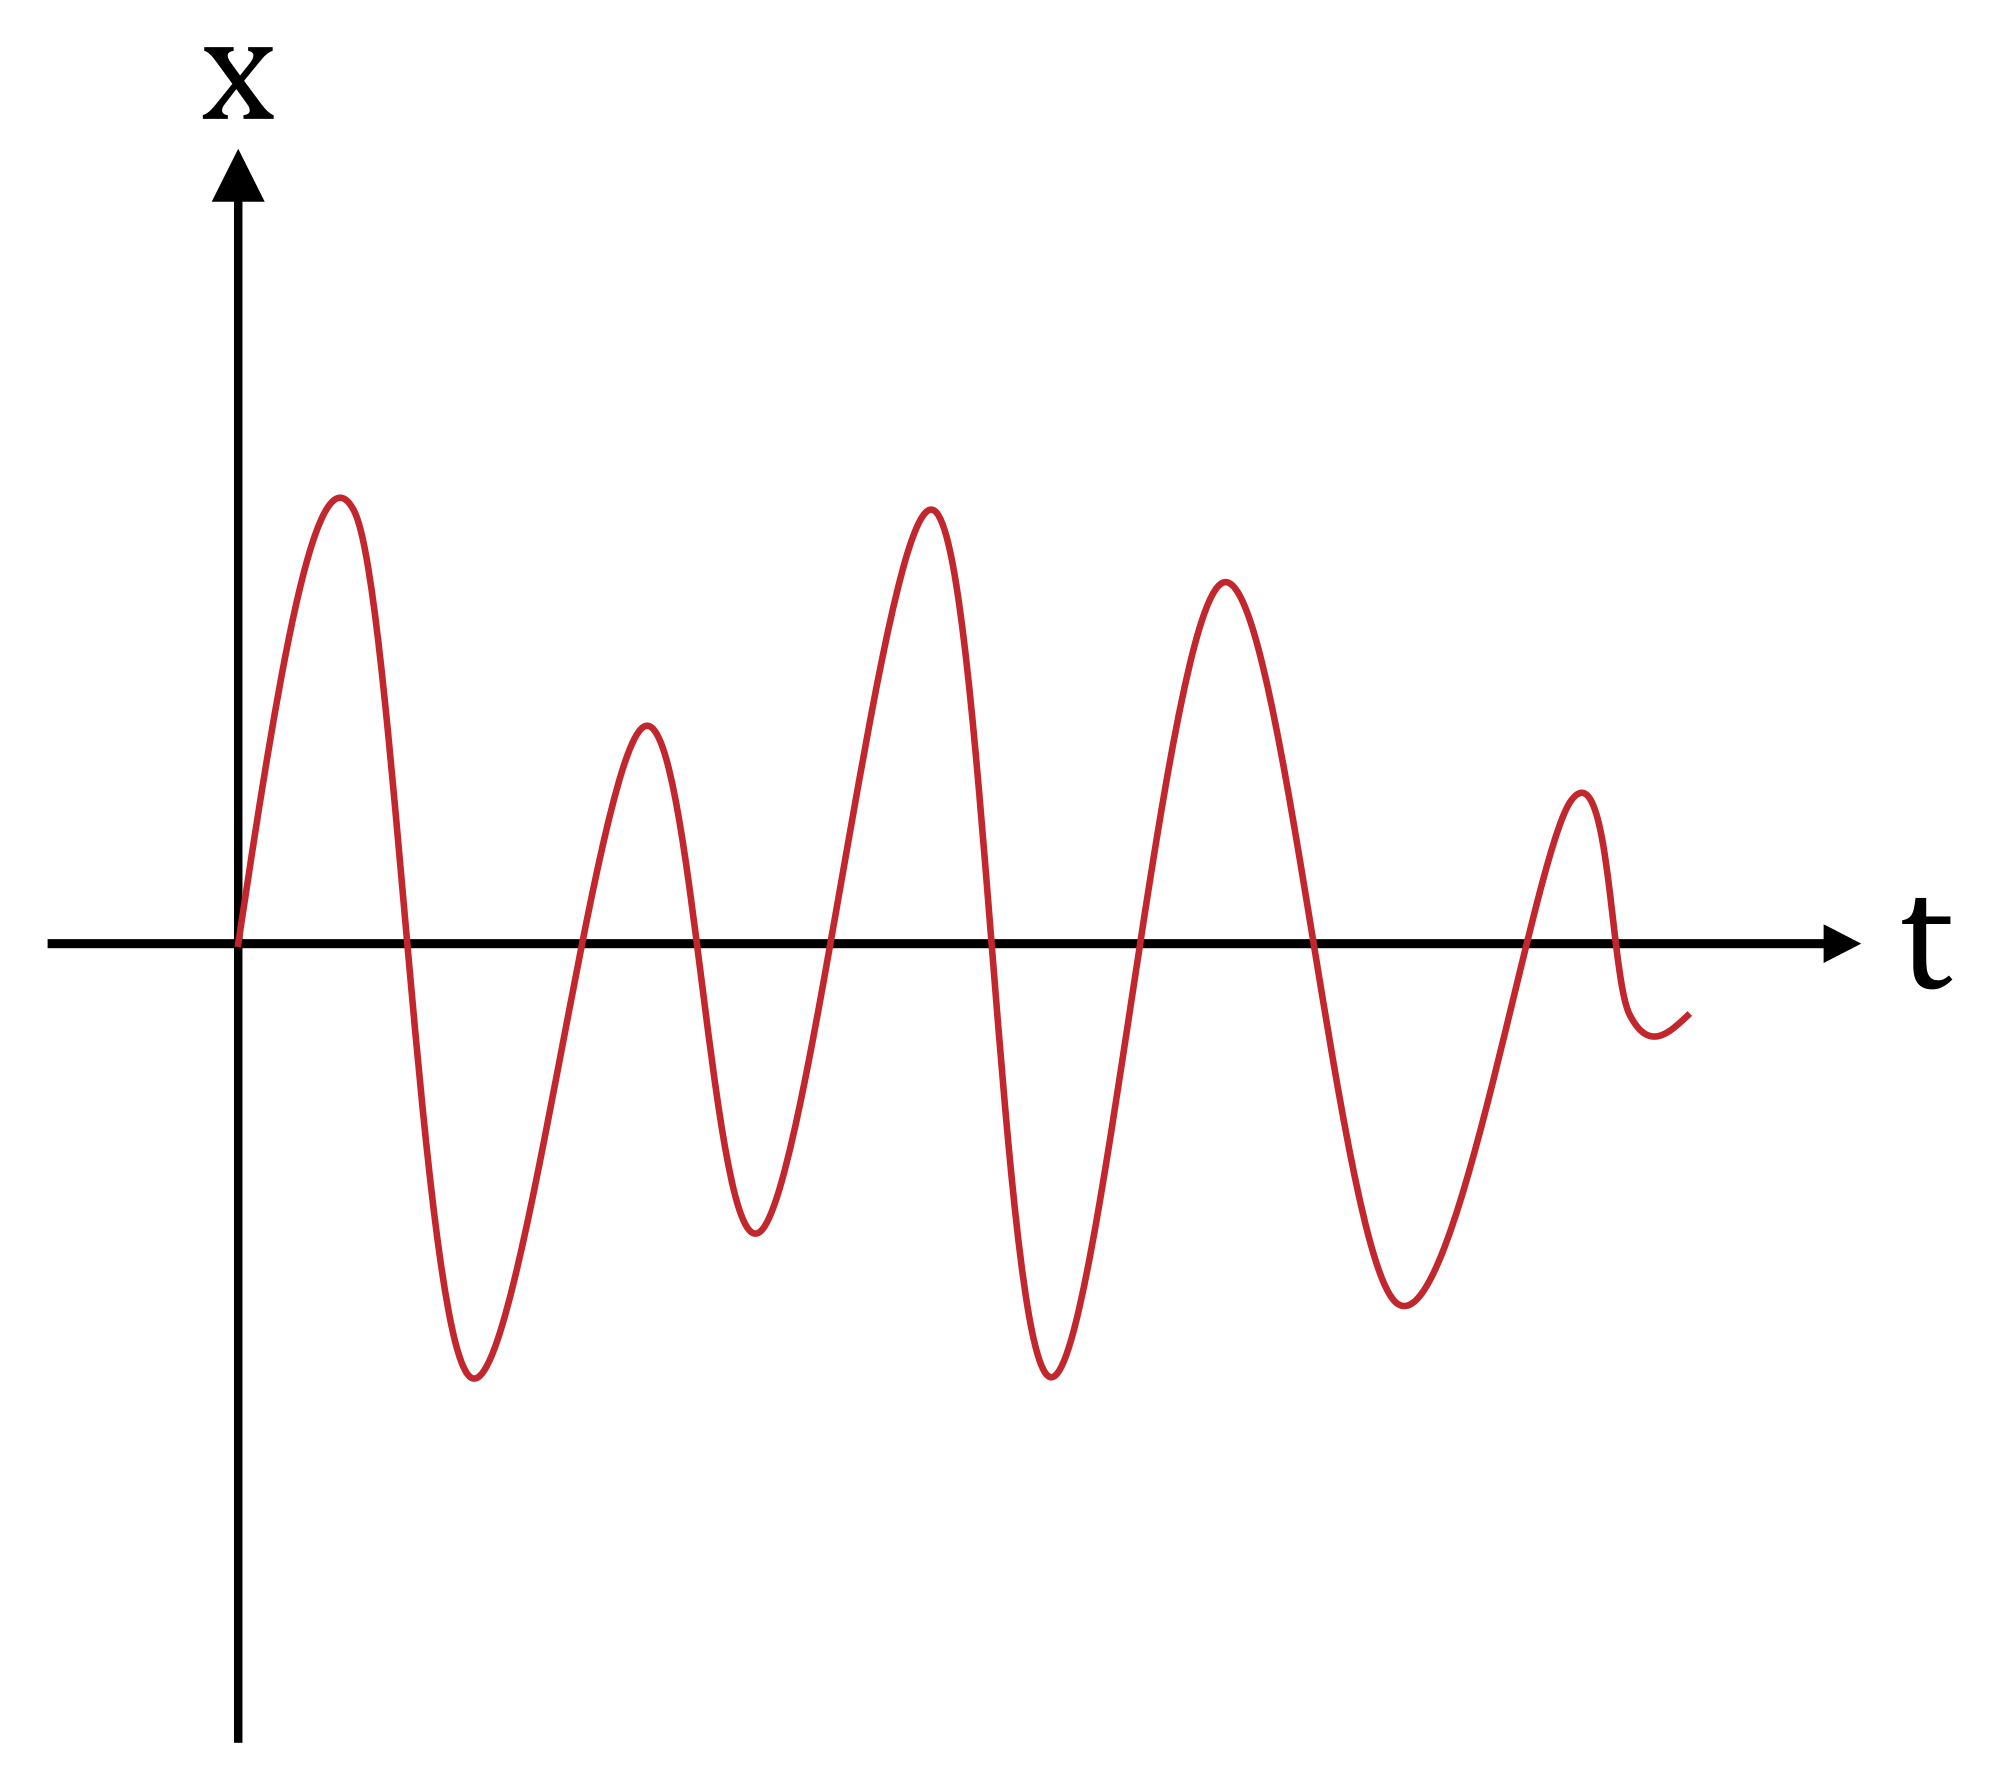
\includegraphics[width=1\textwidth]{analog}
  \caption{Analog Signal}
  \end{figure}
  \end{column}
  \end{columns}
\end{frame}

\begin{frame}\frametitle{Digital Circuit}
  \begin{columns}
  \begin{column}{6cm}
  \begin{itemize}
   \item Discrete Voltage Levels
   \item Is always based on an analog circuit.
   \item Example: Computer
   \item $\Rightarrow$ Binary Numbers

  \end{itemize}


  \end{column}
  \begin{column}{6cm}
  \begin{figure}
  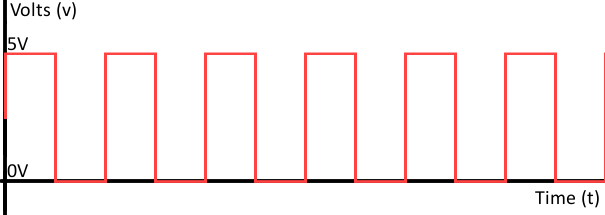
\includegraphics[width=1\textwidth]{digital}
  \caption{Digital Signal}
  \end{figure}
  \end{column}
  \end{columns}
\end{frame}


\section{Binary Numbers}
\begin{frame}\frametitle{Binary Numbers}
  \begin{columns}
  \begin{column}{6cm}
  \begin{itemize}
   \item High Voltage = 1
   \item Low Voltage = 0
   \item Can represent anything from numbers over letters to mp4 videos.
  \end{itemize}

  \end{column}
  \begin{column}{6cm}
  \begin{figure}
  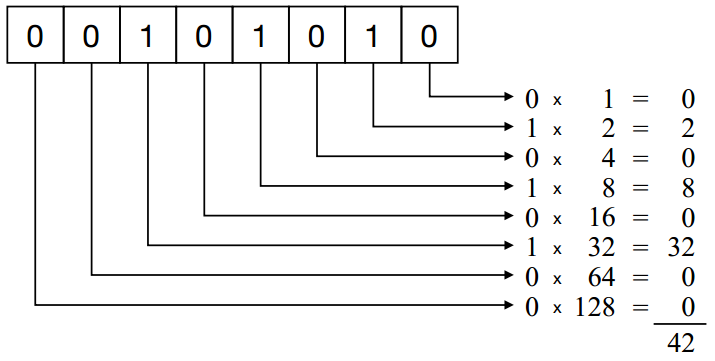
\includegraphics[width=1\textwidth]{binary}
  \caption{Binary Number}
  \end{figure}
  \end{column}
  \end{columns}
\end{frame}


\begin{frame}\frametitle{Binary Numbers}
  \begin{figure}
  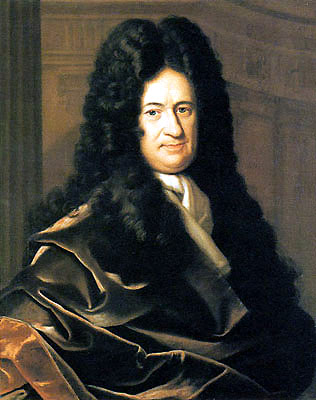
\includegraphics[height=0.7\textheight]{leibniz}
  \caption{Gottfried Leibniz, 1679}
  \end{figure}
\end{frame}


\section{Boolean Algebra}
\begin{frame}\frametitle{Boolean Algebra}
  \begin{columns}
  \begin{column}{6cm}
  \begin{itemize}
    \item \textbf{The conjunction:} $a\land b$ is $1$ if and only if $a$ is $1$ and $b$ is $1$.\\
    \item \textbf{The disjunction:} $a\lor b$  is $1$ if and only if $a$ is $1$ or $b$ is $1$ or both.\\
    \item \textbf{The negation:}  $\overline{a}$ is $1$ if and only if $a$ is $0$.
    \item Associative, Commutative, Distributive, Inverse, Zero
  \end{itemize}
  \end{column}
  
    
  \begin{column}{6cm}
  \begin{table}[H]
  \centering
  \begin{tabular}{c|c||c|c|c}
  \textbf{$a$} & \textbf{$b$} & \textbf{$a\land b$} & \textbf{$a\lor b$} & \textbf{$\overline{a}$} \\ \hline
  0          & 0          & 0            & 0            & 1           \\
  0          & 1          & 0            & 1            & 1           \\
  1          & 0          & 0            & 1            & 0           \\
  1          & 1          & 1            & 1            & 0          
  \end{tabular}
  \caption{truth table}
  \label{tab:truth}
  \end{table}
  \end{column}
  
  \end{columns}
\end{frame}

\section{Truth Tables}
\begin{frame}\frametitle{Truth tables}
  \begin{table}[H]
  \centering
  \begin{tabular}{c|c||c|c|c}
  \textbf{$a$} & \textbf{$b$} & \textbf{$a\land b$} & \textbf{$a\lor b$} & \textbf{$\overline{a}$} \\ \hline
  0          & 0          & 0            & 0            & 1           \\
  0          & 1          & 0            & 1            & 1           \\
  1          & 0          & 0            & 1            & 0           \\
  1          & 1          & 1            & 1            & 0          
  \end{tabular}
  \caption{truth table}
  \label{tab:truth2}
  \end{table}
\end{frame}

\begin{frame}\frametitle{Truth tables}
   \begin{table}[H]
  \centering
  \begin{tabular}{c|c||c|c|c|c|c}
  \textbf{$a$} & \textbf{$b$} & \textbf{$a\land b$} & \textbf{$a\lor b$} & \textbf{$\overline{a}$} & \textbf{ \textcolor{red}{$a==b$}}  & \textbf{ \textcolor{red}{$\overline{a\land  b}\ $}} \\ \hline
  0          & 0          & 0            & 0            & 1          & 1        & 1      \\
  0          & 1          & 0            & 1            & 1          & 0        & 1  \\
  1          & 0          & 0            & 1            & 0          & 0        & 1   \\
  1          & 1          & 1            & 1            & 0          & 1        & 0  
  \end{tabular}
  \caption{truth table}
  \label{tab:truth}
  \end{table}
\end{frame}



\section{Disjunctive Normal-Form}
\begin{frame}
  
  \begin{columns}
  \begin{column}{6cm}
  \begin{itemize}
    \item Let's convert this table in one compact formula!
    \item Disjunctive Normal Form:
    \begin{enumerate}
     \item \textbf{Rows} with logical output \textbf{1}.
     \item Combine inputs with AND. Each row separatly.
     \item Combine rows with logical OR.
    \end{enumerate}

    
    \item Example 1: 
    \begin{itemize}
      \item [\textbf{AND:}]$(a\land b)$
    \end{itemize}
  \end{itemize}
  \end{column}
  
    
  \begin{column}{6cm}
  \begin{table}[H]
  \centering
  \begin{tabular}{c|c||c}
  \textbf{$a$} & \textbf{$b$} & \textbf{$a\land b$} \\ \hline
  0          & 0          & 0      \\
  0          & 1          & 0  \\
  1          & 0          & 0   \\
  1          & 1          & 1 
  \end{tabular}
  \caption{truth table}
  \label{tab:truth}
  \end{table}
  \end{column}
  
  \end{columns}  
\end{frame}


\begin{frame}
  
  \begin{columns}
  \begin{column}{6cm}
  \begin{itemize}
    \item Let's convert this table in one compact formula!
    \item Disjunctive Normal Form:
    \begin{enumerate}
     \item \textbf{Rows} with logical output \textbf{1}.
     \item Combine inputs with AND. Each row separatly.
     \item Combine rows with logical OR.
    \end{enumerate}

    
    \item Example 2: 
    \begin{itemize}
      \item [\textbf{OR:}]$(a\land \overline{b})\lor(\overline{a}\land b)\lor(a\land b)$
    \end{itemize}
  \end{itemize}
  \end{column}
  
    
  \begin{column}{6cm}
  \begin{table}[H]
  \centering
  \begin{tabular}{c|c||c}
  \textbf{$a$} & \textbf{$b$} & \textbf{$a\lor b$} \\ \hline
  0          & 0          & 0      \\
  0          & 1          & 1  \\
  1          & 0          & 1   \\
  1          & 1          & 1 
  \end{tabular}
  \caption{truth table}
  \label{tab:truth}
  \end{table}
  \end{column}
  
  \end{columns}  
  
  
  
\end{frame}


\begin{frame}
  
  \begin{columns}
  \begin{column}{6cm}
  \begin{itemize}
    \item Let's convert this table in one compact formula!
    \item Disjunctive Normal Form:
    \begin{enumerate}
     \item \textbf{Rows} with logical output \textbf{1}.
     \item Combine inputs with AND. Each row separatly.
     \item Combine rows with logical OR.
    \end{enumerate}

    
    \item Example 3: 
    \begin{itemize}
      \item [\textbf{==:}]$(\overline{a}\land \overline{b})\lor(a\land b)$
    \end{itemize}
  \end{itemize}
  \end{column}
  
    
  \begin{column}{6cm}
  \begin{table}[H]
  \centering
  \begin{tabular}{c|c||c}
  \textbf{$a$} & \textbf{$b$} & \textbf{$a == b$} \\ \hline
  0          & 0          & 1      \\
  0          & 1          & 0  \\
  1          & 0          & 0   \\
  1          & 1          & 1 
  \end{tabular}
  \caption{truth table}
  \label{tab:truth}
  \end{table}
  \end{column}
  
  \end{columns}  
  
  
  
\end{frame}







\section{Drawing a circuit}

\begin{frame}
  \begin{figure}[H]
\centering
  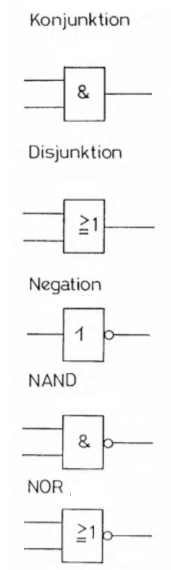
\includegraphics[height=0.6\textwidth]{logic_symbols}%
  \caption{Logic circuit symbols}%
  \label{fig:logic_symbols}
\end{figure}
\end{frame}


\begin{frame}
  \begin{columns}
  \begin{column}{5cm}
  Disjunctive normal-form for the equivalence: 
  \newline\newline
  $(\overline{a}\land \overline{b})\lor(a\land b)$
  \end{column}
  
  \begin{column}{6cm}
    \begin{figure}[H]
      \centering
      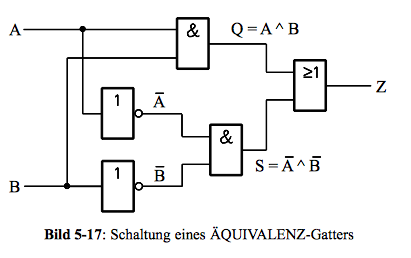
\includegraphics[width=1\textwidth]{equivalence}%
      \caption{Example for circuit design: the equivalence}%
      \label{fig:equivalence}
    \end{figure}
  \end{column}
  \end{columns}  
\end{frame}


\begin{frame}
  \begin{columns}
  \begin{column}{5cm}
  Now let's make it easier: Use only NAND's!
  \newline\newline
 % $(\overline{a}\land \overline{b})\lor(a\land b)$
  \end{column}
  
  \begin{column}{6cm}
    \begin{figure}[H]
      \centering
      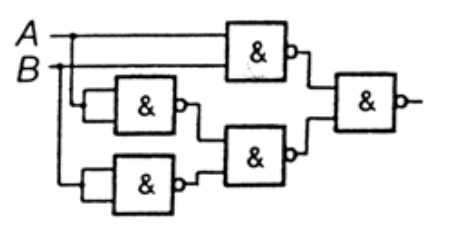
\includegraphics[width=1\textwidth]{equivalence_optimized}%
      \caption{Optimized equivalence circuit}%
      \label{fig:equivalence_optimized}
    \end{figure}
  \end{column}
  \end{columns}  
\end{frame}


\begin{frame}
  \begin{columns}
  \begin{column}{5cm}
  Now let's make it easier: Use only NAND's!
  How?
  \newline\newline
 % $(\overline{a}\land \overline{b})\lor(a\land b)$
  \end{column}
  
  \begin{column}{6cm}
    \begin{figure}[H]
      \centering
      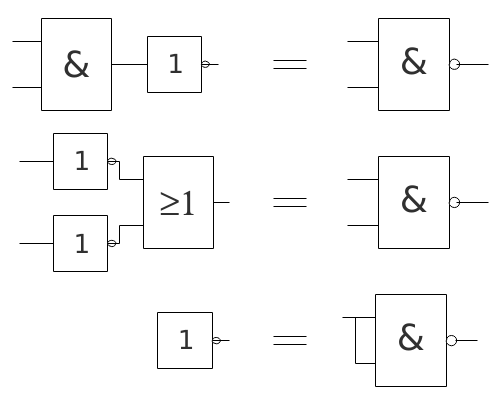
\includegraphics[width=1\textwidth]{nand_conversion}%
      \caption{NAND Conversion}%
      \label{fig:equivalence_optimized}
    \end{figure}
  \end{column}
  \end{columns}  
\end{frame}





\section{Combinatoric Circuits}
\section{Sequential Circuits}







\end{document}